\scanpage{44}
\mspage{1}
\uline{Groupoïdes de Teichmüller}.

\textcircled{1} Cas topologique.

La variante la plus simple est
\[
\mathcal T^+_{\mathrm{top}}\quad\text{ou}\quad\mathcal T_{\mathrm{top}}
\]
(\uline{groupoïde de Teichmüller} \uuline{orienté} \uline{topologique})

\uline{objets} : surfaces \uline{à bord} compactes orientées $(\Sigma)$\unsure{,|.}

\uline{flèches} : classes d'isotopie d'iso (conservant l'orientation)

\margin{Finalement, tant qu'on ne travaille pas au point de vue
arithmétique, il semble que c'est le gros $\mathcal T^\pm$ qui sera
le plus utilisé; \deleted{\unsure{tout|d'où}} c'est lui qui
mérite donc ici la notation la plus simple $\mathcal T$,
et le \unsure{gr.\ or.} orienté de s'appeler $\mathcal T^+$.}

Variante immédiate
\[
\mathcal T_{\mathrm{top}}^\pm
\]
(\uline{groupoïde de Teichmüller} \uuline{biorienté} \uline{topologique}) :
mêmes objets, flèches sont les classes d'isotopie d'homéomorphismes
(ne conservant pas néc\textsuperscript{t}. l'orientation).

Soit $[\pm1]$ le groupoïde ayant un seul objet $e$ (par exemple $e=\varnothing$)
et comme groupe d'autom $\pm1$. On a un morphisme de signature
\diagram{\begin{tikzcd}[ampersand replacement=\&]
\mathcal T^\pm_{\mathrm{top}}\arrow[r,"\chi"]\&{[\pm1]}
\end{tikzcd}}
dont la \uline{fibre} \deleted{\unsure{est}} (ou noyau) est
$\mathcal T_{\mathrm{top}}^+=\mathcal T_{\mathrm{top}}$.
\margin{\figure{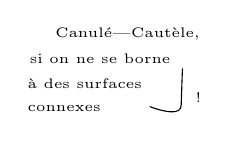
\begin{tikzpicture}[x=0.27cm,y=0.30cm,every node/.style={anchor=west,inner sep=0pt,outer sep=0pt,font=\tiny}]
\node at (1.2,0) {\unsure{Canulé|Cautèle},};
\node at (0,-1.05) {si on ne se borne};
\node at (-0.1,-2.12) {à des surfaces};
\node at (-0.1,-3.18) {connexes};
\node at (7.8,-2.72) {!};
\draw (7.18,-1.46) -- (7.12,-3.02)
  .. controls (7.13,-3.47) and (6.28,-3.30) .. (5.64,-3.08);
\end{tikzpicture}}}

La variante la plus complexe est
\[
S_*\mathcal TD_{\mathrm{top}}^+\quad\text{ou}\quad
S_*\mathcal TD_{\mathrm{top}},
\]
``\uline{groupoïde de Teichmüller} \inserted{\uline{orienté}}
\uline{spécial dévissé topologique}''
\margin{43}
